\documentclass{article}
\usepackage{graphicx}
\usepackage[ampersand]{easylist}
\usepackage{fullpage}

%\usepackage[hidelinks]{hyperref}
\usepackage{hyperref}
\usepackage{xcolor}
\hypersetup{
	colorlinks,
	linkcolor={red!50!black},
	citecolor={blue!50!black},
	urlcolor={blue!80!black}
}
\usepackage{booktabs}
\usepackage[T1]{fontenc}


\begin{document}

\title{Simulation Documentation}
\author{Michael McDonnell}

\maketitle
%TOC?

\tableofcontents
\newpage

\section*{Overview}
\addcontentsline{toc}{section}{Overview}

\subsection*{Background}
\addcontentsline{toc}{subsection}{Background}

This simulation was developed to generate data for a system that uses computer vision to identify and track road features such as intersections using a single vehicle mounted camera. The simulation developed is lightweight in that the functionality is only as much as is required for the computer vision system data generation which consists of a camera image feed from a vehicle driving in simulation. A significant challenge in the development of this simulation was the Inter Process Communications (IPC) implementation which allowed direct communication of data (image data and server messages) between the Unity simulation and a Python process running in the background.

Despite the somewhat narrow focus, the simulation as developed allows for significant extension. Several difficult challenges have been solved and extension options are discussed at applicable points. It is hoped that this documentation will provide enough context and understanding to be able to follow the operation of the simulation and extend on it as required.

\subsection*{Unity}
\addcontentsline{toc}{subsection}{Unity}

The simulation is developed in Unity and some familiarity with the Unity engine is required to gain a full understanding of how the system works, especially if the intent is to modify or extend the system. Unity uses C\# as a scripting language and a component based approach to organisation. A central \textbf{MonoBehaviour} class provides interface with engine functions (such as initialisation and update functions) and facilitates attaching scripts to \textbf{Game Objects} in the scene to allow the script logic to function. 

The engine allows full use of `pure' C\# however and many of the data classes used in simulation were implemented without extending from the Unity \textbf{MonoBehaviour} class. There are a raft of official and non official resources for learning Unity with a recommended starting point being the official tutorials at \url{https://learn.unity.com/}. 

\section{Project setup}

The project was developed using Unity 2019.1.4f1 however only uses general engine functionality so there should be no issues arising from using other Unity versions. As always, make a backup just to be safe before changing versions. The grass texture used was `ground4' from ADG\_Textures, Ground Volume 1 \footnote{Available from the Unity Asset Store at:  \url{https://assetstore.unity.com/packages/2d/textures-materials/floors/outdoor-ground-textures-12555} } which is a free texture pack and the vehicle used is the Sedan from NWH Vehicle Physics \footnote{Available (for purchase) from the Unity Asset Store at: \url{https://assetstore.unity.com/packages/tools/physics/nwh-vehicle-physics-107332}. Only the vehicle model was used from this package; no control logic has been included. }. These assets (texture and model) do not affect the simulation and can be changed as desired.

IPC detail is included in section \ref{s:ipc} however at this stage it will be noted that an additional non-Unity file is included. \textbf{PythonZMQServer.py} is a ZeroMQ server process that is launched prior to the simulation attempting to initialise IPC. This process runs in the background and waits for communications from the simulation process.

\begin{figure}[h!]
	\centering
	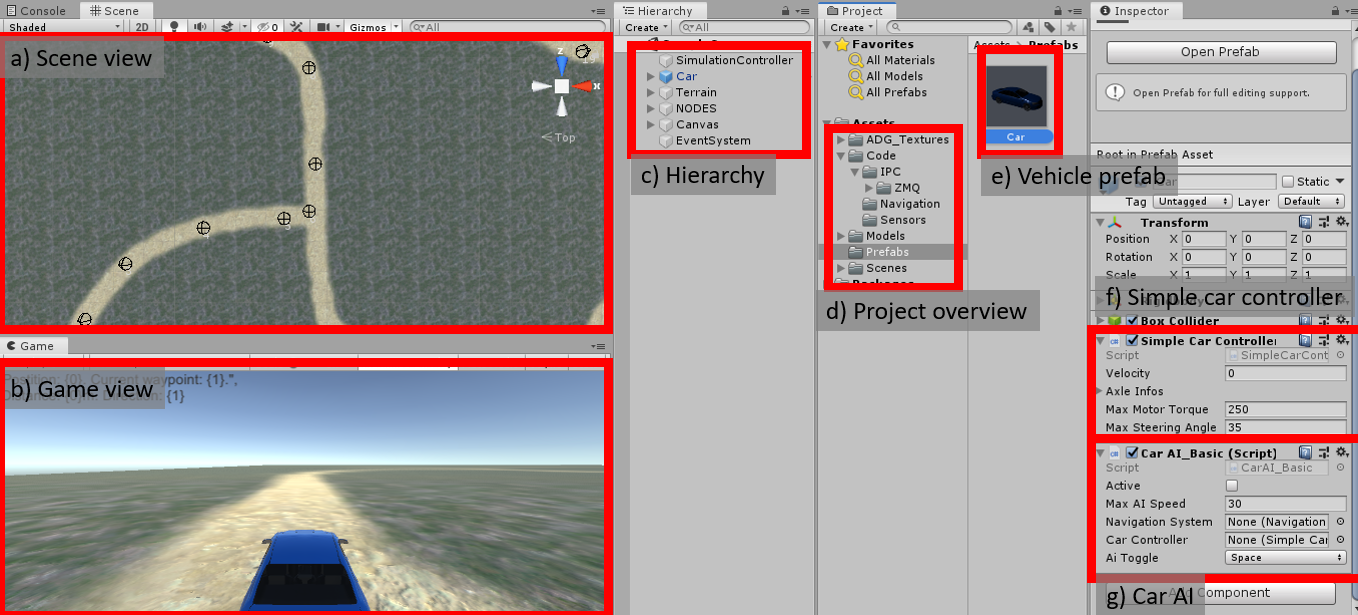
\includegraphics[width=0.95\linewidth]{projectOverviewAnnotated.png}
	\caption{Simulation Results}
	\label{projectOverviewAnnotated}
\end{figure}


A view of the project setup in Unity is included as figure \ref{projectOverviewAnnotated}. Details in this figure are as follows:
\begin{easylist}[itemize]
	& \textbf{a) Scene view.} This is the `editor' view of the scene. In this figure the camera is positioned high over the test area looking down. Editor visualisations known as `gizmos' are visible (black wireframe spheres) marking waypoints on the road.
	& \textbf{b) Game view.} This is the view a player in game would see. The player camera is high and behind the vehicle. Note this is \textbf{not} the camera that is used to generate image data. 
	& \textbf{c) Hierarchy.} This contains all items in the current scene. The \textit{Car} object is coloured indicating it is an instance of a prefab.
	& \textbf{d) Project overview.} This region shows the folder structure of the project.
	&& The \textit{Code} folder is visible here. This folder contains all the scripts with the simulation logic. In this figure it is fully expanded showing the main subfolders (IPC, Navigation, Sensors)
	&& The current selected folder is \textit{Prefabs}
	& \textbf{e) Vehicle prefab.} This is the sole prefab in the \textit{Prefabs} folder. The vehicle inside the scene is an instance of this.
	& \textbf{f) Simple car controller.} This is a MonoBehaviour script is on the vehicle prefab (thus also on the instance of the vehicle in the scene) and contains the physics logic required for the vehicle to move. This is a simple script based on Unity documentation \footnote{Based on \url{https://docs.unity3d.com/Manual/WheelColliderTutorial.html}} and represents a minimum simulation of vehicle movement.
	& \textbf{g) Car AI.} Another MonoBehaviour script (or component) which contains the AI logic. This is discussed in section \ref{s:AI}.\\
\end{easylist}


The waypoints visible in the Scene view are managed by the \textbf{NodeVisualiser} class. This represents an example series of waypoints for a vehicle to follow and placement logic is based off road nodes as used in Google Maps and Open Street Maps data structures. Nodes are simply empty Game Objects that are positioned in the scene view. The order of waypoints generated by these nodes is determined by the order in the hierarchy of the Game Objects. The \textbf{NodeVisualiser} handles visualisation and waypoint consolidation and provides a list of waypoints to the Navigation System\footnote{This class is suitable for refactoring into a NodeVisualiser class solely responsible for visualisation and a WaypointManager class which handles navigation system testing. It was not deemed necessary for the original use case but is recommended if this aspect is extended.} (discussed further in section \ref{s:AI}). This script simply gets the list of all \textit{NODES} Game Object children and creates a List of \textbf{RoadNode} based on the individual Game Object positions. These are visualised using editor gizmos via the \textbf{OnDrawGizmos} MonoBehaviour function.

\section{General Logic}

In area c) of figure \ref{projectOverviewAnnotated} the top Game Object is \textit{SimulationController}. This object contains two components; \textbf{SimulationController} and \textbf{ImageSensorClient}. The latter is discussed in section \ref{s:ipc}. As outlined previously, the vehicle has a \textbf{CarAI\_Basic} component which is responsible for the input to the vehicle controls.

A \textbf{DebugUpdater} script is included which provides some debug information and visualisation. This script provides a text output of the GPS data (see section \ref{s:sensors}) and draws an editor gizmo line to the current waypoint.

\subsection{Simulation control}

Control of the simulation is managed by the \textbf{SimulationController} class. This class manages individual simulation `ticks' and includes tick start and complete events. The simulation has a \textbf{DoNextTick} method which is called by the \textbf{ImageSensorCommunicator} as discussed in section \ref{s:ipc}. This class includes a public \textit{tickLength} variable which is used to determine when to stop simulating. When \textit{tickLength} seconds have elapsed after \textbf{DoNextTick} is called, the \textbf{SimulationController} sets the simulation time scale to 0. On \textbf{DoNextTick} the time scale is reset to 1.0 which results in another \textit{tickLength} second simulation.

\subsection{Vehicle control}

The \textbf{CarAI\_Basic} component is a simple script which sets the motor (positive to accelerate, negative to brake) and steer (-1.0 to 1.0 representing full left to right). These values are passed to the \textbf{SimpleCarController} component which handles the physical movement of the vehicle. The vehicle physics are implemented using Wheel Colliders controlled by the \textbf{SimpleCarController} component. Discussion of Wheel Collider control is outside the scope of this documentation however is outlined in the Unity Manual.

The \textbf{CarAI\_Basic} includes a flag which toggles via keypress (defaults to SPACEBAR) between player control and AI control of the car. Player control is simply WASD or Arrow keys to accelerate/brake and steer. AI control is discussed further in section \ref{s:AI}.


\section{Sensors} \label{s:sensors}

The `image sensor' or camera was implemented initially as a standalone class which incorporated the IPC logic. This was suitable for the initial purpose however a general sensor definition was created to allow further extension. Future work can include separating the sensor and communication logic from the existing \textbf{ImageSensorClient} and \textbf{ImageSensorCommunicator} classes (discussed in section \ref{s:ipc}) to a specific IPC manager and a new camera sensor class.

A generic `sensor' was implemented using a \textbf{Sensor} interface. This contains a single \textbf{Tick} method which returns \textbf{SensorData}. \textbf{SensorData} is an abstract class which acts as a data container for sensor data. This rather simple initial definition allows a generic implementation of sensor types. As additional interface control is identified it can be expanded if required. 

\subsection{GPS}

An example GPS sensor was implemented which demonstrates the usage of the `sensor' concept. The sensor is a MonoBehaviour (that is, attached to a Game Object) which implements the \textbf{Sensor} interface. This class implements the \textbf{Tick} method which is called externally. The GPS sensor stores the previous position as a class variable and each \textbf{Tick} calculates the speed (change in position over the tick time) and updates the position. This information is stored in a \textbf{GPSData} class (which extends \textbf{SensorData}) and is returned on each tick.

The GPS sensor also includes a \textit{GPSTickEvent} which external classes can subscribe to in order to receive a copy of the \textbf{GPSData} when the sensor `ticks'.

\subsection{Extension sensors}

The GPS sensor represents a simple implementation of the generic sensor definition and can be used as a starting point for other sensors. As an example a laser distance sensor (\textbf{LaserSensor}) implementation may use the Game Object orientation and position to define the laser direction and position and each \textbf{Tick}, fire a raycast and return a simple \textbf{LaserData} class which contains the distance to the ray hit location.

The use of `on tick' events is encouraged as it allows integration of more complex logic to the existing sensors. An example of this is the navigation system discussed in section \ref{s:AI}.

\section{AI driver}\label{s:AI}

The AI vehicle control uses a very simplistic approach to waypoint navigation using a navigation system. The AI control uses the distance to next waypoint to determine a target motor speed and uses the direction vector to the next waypoint to set the steering angle directly. While this system is very simplistic it provides an effective initial implementation of waypoint based driving using navigation system logic.

\subsection{Navigation}

The navigation system relies on two supporting data structures. These are merely wrappers for existing data structures currently but this allows for ease of extension in future: 
\begin{easylist}
	& \textbf{RoadNode}. A simple data struct which contains a Vector3 for the node position.
	& \textbf{NavigationRoute.}  A simple data struct which contains a List of node positions representing route waypoints.
\end{easylist}

The Navigation system is contained in the \textbf{NavigationSystem} class which contains relatively simple logic with event based implementations. The navigation system requires a GPS sensor (on the same object or a child of the navigation system object). The navigation system subscribes to the GPS `on tick' event and uses that data to update internal navigation positional data. For this simple implementation, the navigation system has a series of waypoints set by the \textbf{NodeVisualiser} class as previously discussed.

The navigation system uses position updates to determine proximity to the current waypoint target. If the distance is within a threshold, the navigation system will update to the next waypoint. Events are thrown on arrival at a node, on setting a new node active and on completing the navigation route. The system also includes a helper method to get a direction vector to the current waypoint node.

Note that this represents an example implementation of a system that interacts with sensors as defined. It is fully functional and is used by the AI driving system. Not all of the events that are declared and raised are currently subscribed to however they demonstrate an effective option to allow complex interactions while remaining decoupled. An example of a further extension to this system would be to store a graph of all nodes and integrate a pathfinding system to allow external input to set a destination node rather than rely on a pre-specified route to travel.

\section{Inter Process Communication (IPC)}\label{s:ipc}

IPC is achieved using ZeroMQ (ZMQ). The ZMQ documentation is located at \url{http://zguide.zeromq.org/page:all} with examples in a range of languages including C, C++, Python and C\#. The minimal architecture outlined at \url{https://github.com/off99555/Unity3D-Python-Communication} was used as a starting point to develop the communication. IPC was implemented in the simulation by a Python ZMQ server script running in the background which accepts camera image data and commands the next simulation tick. A C\# ZMQ client runs within the Unity process and opens a connection to the server when the simulation is triggered to send image data. It should be noted that the Python server was implemented as additional processing was undertaken within Python however any language with a ZMQ wrapper can be used for the server. Additionally ZMQ is multi transport and includes TCP-IP and UDP so, while this implemented a local `server' for IPC, this same implementation can scale quite simply to remote server communications. 

The \textbf{ImageSensorCommunicator} class is the C\# class which extends \textbf{RunAbleThread} which is responsible for packaging the image data into the required byte array and sending to the server. In the lightweight simulation developed the information flowing \textit{from} the simulation is just the current camera frame at the end of the simulation tick and the information \textit{to} the simulation is just "\textbf{Ack}" (run the next simulation tick) or "\textbf{END}" (end the client communication). This class triggers the next simulation tick by calling the \textbf{DoNextTick} method on the \textbf{SimulationController} instance.

This implementation was suitable for the generation of data required however provides the basic framework for generalisation and extension. Currently this class handles the response from the server and triggers the next simulation 'tick'; in a more robust application an overall sensor communication manager should be implemented which will centralise simulation ticks and messages. Additionally, extending the control the server has over the client simulation is quite simple. In lieu of the simple string based messaging system currently used, standardising the first \textbf{B} bytes as the message instruction with the remainder of the message as data would allow control over any aspect of the simulation. 


\subsection{Code}

The plugins located within the \textit{Code/IPC/ZMQ/Plugins} folder are \textbf{AsyncIO} and \textbf{NetMQ} and are required for ZeroMQ to function. Additional code located within \textit{Code/IPC/ZMQ} is as follows:

\begin{easylist}[itemize]
	& \textbf{RunAbleThread} - This is a base class for sensor communication to inherit from and is used under MIT license from \url{https://github.com/off99555/Unity3D-Python-Communication}. This provides the framework which allows child classes to execute ZeroMQ networked code inside a \textbf{Run} method.
	& \textbf{ImageSensorCommunicator} - Extends \textbf{RunAbleThread} to implement simulation specific communication. Initialises connection with server and sends image sensor data as it becomes available.
	& \textbf{ImageSensorClient} - This class handles the generation of image sensor (camera) data and the initialisation and updating of data for the \textbf{ImageSensorCommunicator}.
	& \textbf{PythonZMQServer.py} - \textit{This file is included external to the Unity project but is addressed here due to relevance.} Python process that also implements ZMQ. This file must be running in the background before the simulation system attempts to establish IPC. This acts as the ZMQ server which listens for simulation system messages and replies with "Ack", triggering the next simulation tick, or "END", which is the trigger for the Unity simulation to stop sending data. The ending criteria is specified in this file as a total number of images received. This file also manages naming and saving images that are received from the simulation. 
\end{easylist}



\subsection{Example Instruction-Variable communications specification}

While the simulation as developed did not implement a robust instruction set, a basic architecture and specification was developed which would allow it. The logic developed included the ability to spawn objects in simulation at runtime and set individual object parameters (including setting desired control inputs for vehicles). This general approach can be extended almost indefinitely for fine grained control as needed. The developed concept is presented here in order to provide a starting point for more robust extensions. The modifications to the current architecture are as follows:

\begin{easylist}[itemize]
	& The simulation manager (or similar) is populated with an array of all spawnable prefabs
	&& Spawnable prefabs implement an interface \textit{ISimulationObject} which includes methods for communicating with simulation objects
	&& At the minimal level described here, \textit{ISimulationObject} has a method \textbf{SetVariables} which accepts an array of bytes representing a portion of the server message.
	& The simulation manager creates a Dictionary <ushort, ISimulationObject> which contains all objects in simulation indexed by ID (ushort corresponding to a two byte ID). 
	&& Note that this implementation is as a dictionary due to the server assigning the object ID which means IDs may not be contiguous. Alternate implementations may involve the simulation providing an object ID (which is communicated to the server) however this approach was adopted for initial simplicity. The system as presented does not do ID collision checking; some form of insurance against duplicate IDs will need to be implemented.
\end{easylist}


An example of how to extend the Simulation-Server communication is to implement an initial 2 byte instruction followed by expected instruction arguments. Table \ref{tab:commsInstructionDemo} includes an example instruction set which will be used to demonstrate the logic. In this instance each message from the server will have a minimum size of 2 bytes.


\begin{table}[h!]
	\centering
	\begin{tabular}{@{}ccc@{}}
		\toprule
		\textbf{Instruction code} & \textbf{Instruction}          & \textbf{Data}                                                                                                                        \\ \midrule
		0x00                      & Stop simulation               & Nil                                                                                                                                  \\
		0x01                      & Next simulation tick          & Nil                                                                                                                                  \\
		0x02                      & Spawn new object              & \begin{tabular}[c]{@{}c@{}}Spawn prefab ID (2 bytes)\\ Instance ID (2 bytes)\\ Spawn coordinates [x (float), y (float)]\end{tabular} \\
		0x0A                      & Set object variables          & \begin{tabular}[c]{@{}c@{}}Instance ID\\ Object variable data\end{tabular}                                                           \\
		0x1E                      & Save current simulation state & Nil                                                                                                                                  \\ \bottomrule
	\end{tabular}
	\caption{Example implementation of instruction-argument communications protocol}
	\label{tab:commsInstructionDemo}
\end{table}

On message receipt, the first two bytes are extracted which represents the instruction to process. This value is used to look up an instruction to run which may extract additional data from the message if required. Each instruction (implemented in C\#) will expect different message data with some only expecting the instruction while others will expect additional arguments in the bytestream message.
As an example, if the first two bytes are 0x00, the simulation will stop. If the first two bytes are 0x01, the 'next tick' command will run. These instructions are immediately executed without requirement for additional information. Another example of this is if the first two bytes are 0x1E, the simulation save instruction will be called and no further data will be expected in that message.



The following subsections illustrate by example how messages may be processed.

\subsubsection {Message data: 0x1E}
The first two bytes (0x1E) correspond to the \textit{Save current simulation state }instruction. The simulation state is saved to disk and no further data is expected from the message.

\subsubsection {Message data: 0x02400C42FB3333420747AE}

The first two bytes (0x02) correspond to the \textit{Spawn new object }instruction. As per table \ref{tab:commsInstructionDemo} we know the data will be the prefab ID (2 bytes), instance ID (2 bytes) and the x and y coordinates (two 64 bit (8 byte) floating point numbers). Using the message the process then could be:
\begin{easylist}[itemize]
	& Extract the next two bytes (0x40) which is the prefab ID. This value can be used to `look up' the prefab in a static array and instantiate the object.
	& Extract the next two bytes (0x0C) and set the spawned instance ID to this number. This instance can then be added to a dictionary using the ID as the key.
	& Extract the next four bytes (0x42FB3333) and temporarily store for the x coordinate
	& Extract the next four bytes (0x420747AE) and temporarily store for the y coordinate
	& Set the spawned object position to the position represented by the temporary x and y values\\
\end{easylist}


\subsubsection {Message data: 0x0A0D13F3333332BE4CCCCD}

The first two bytes (0x0A) correspond to the \textit{Set object variables }instruction. As per table \ref{tab:commsInstructionDemo} we know the data will be the instance ID (2 bytes) followed by object variable data. In this case the object ID is 0x0D so the instance of this object is retrieved using a dictionary or similar. As each object instance will implement relevant instruction interfaces, we can then pass the remaining message data (0x13F3333332BE4CCCCD) to a SetVariables method on the object. In this example, the object is a vehicle in simulation.

The SetVariables method on the object would use a similar approach; using the provided remaining message data the process could be:
\begin{easylist}[itemize]
	& Extract the first byte of data (0x1) and use this value to determine the variable to be set (for example via a switch statement). The type of this variable will determine the number of bytes to extract next. In this example this value corresponds to the steering angle which is a value between -1.0 and 1.0. In this example the steering angle is a 64 bit floating point number so we require 8 bits.
	& The next 8 bits are extracted (0x3F333333) and the value (0.7) is set to the steering angle.
	& As there is more data remaining, the next byte (0x2) is extracted to determine the next variable to be set. This corresponds to acceleration which is also an 8 bit variable so 8 more bits (0xBE4CCCCD) are extracted and the resulting value (-0.2) is set as the acceleration.
\end{easylist}



\section*{Concluding remarks}
\addcontentsline{toc}{section}{Concluding remarks}

This simulation provides an initial implementation of basic IPC, AI driving and sensor systems. The simulation provided effective outputs based on the original requirements however has the capacity to be significantly extended in all three areas. The detail provided here should allow an interested reader to understand the logic of the system and how to go about extending the system for their own purposes.

\end{document}